\thispagestyle{lichsutoanhocnone}
\pagestyle{lichsutoanhoc}
\graphicspath{{../lichsutoanhoc/pic/}}
\everymath{\color{lichsutoanhoc}}
\blfootnote{$^1$\color{lichsutoanhoc}Cộng tác viên Viện Toán học.}
\begingroup
\AddToShipoutPicture*{\put(0,616){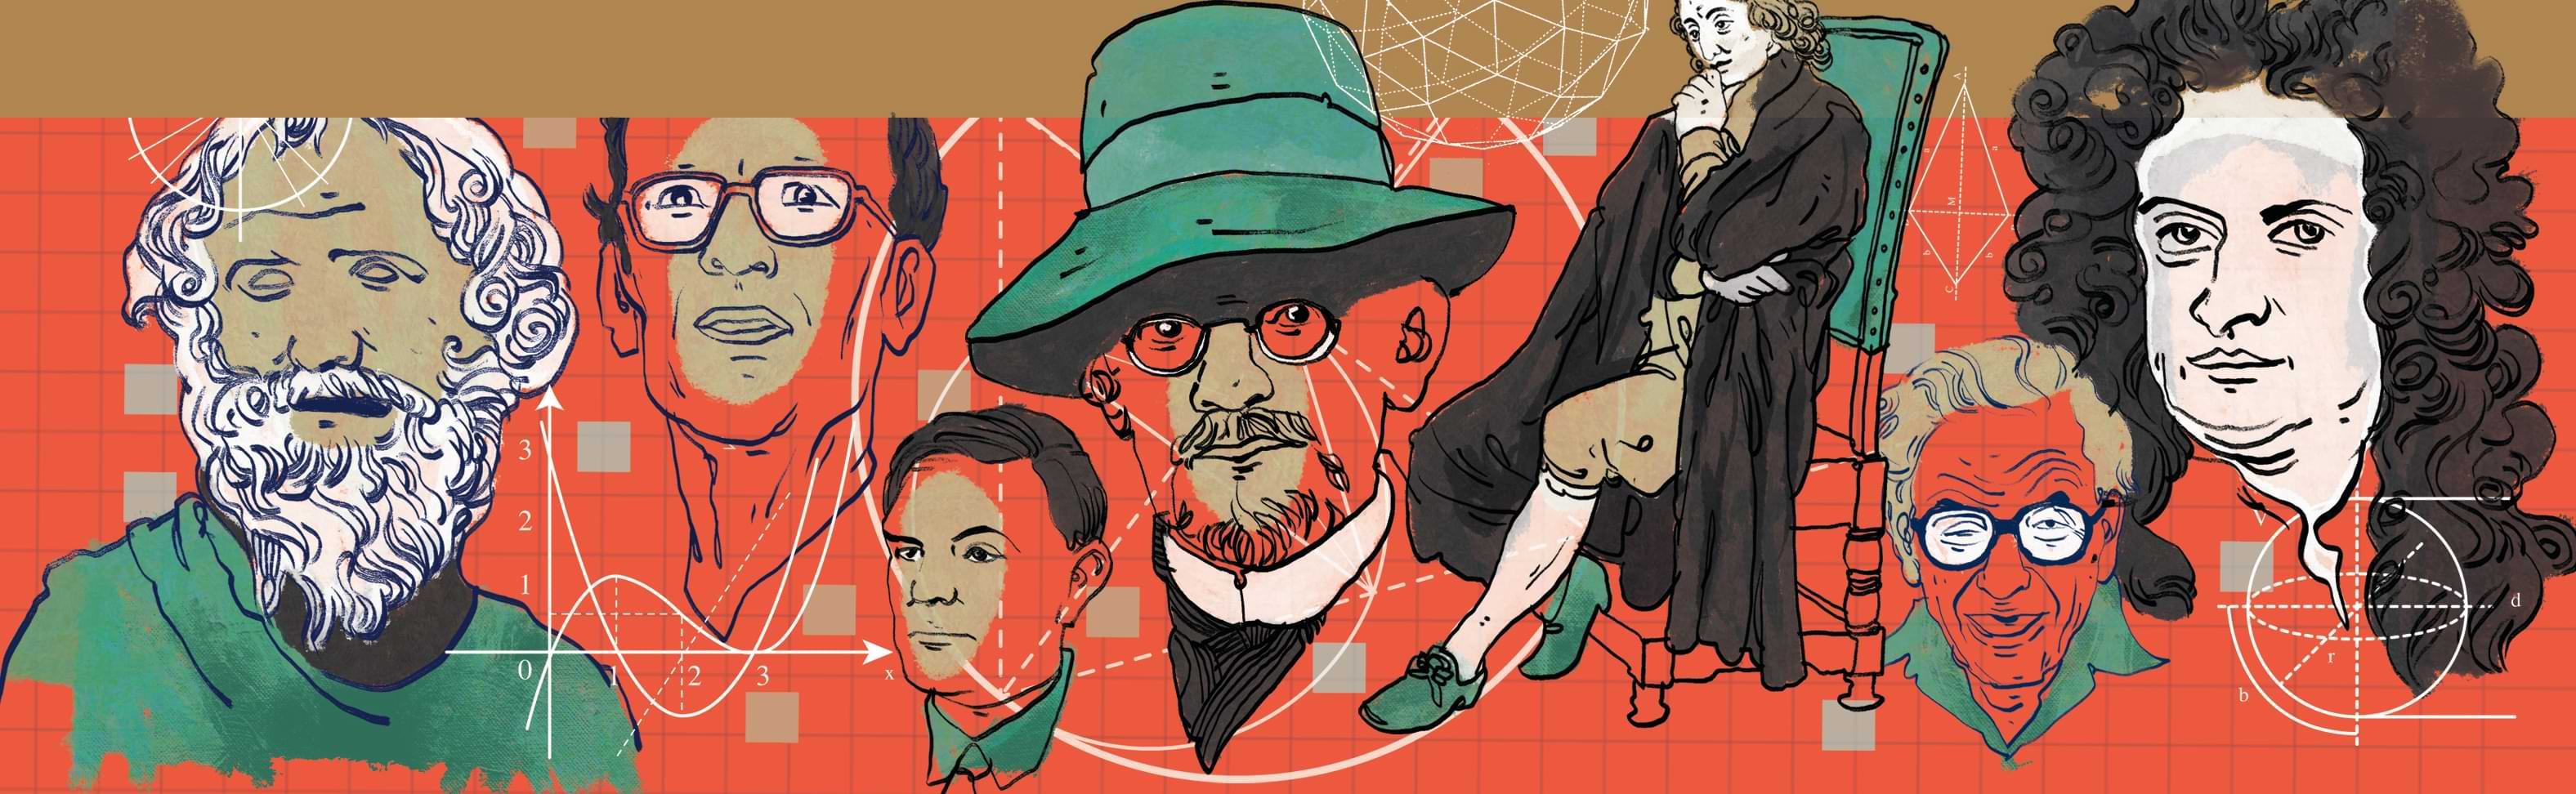
\includegraphics[width=19.3cm]{../bannerlichsu}}}
\AddToShipoutPicture*{\put(58,469){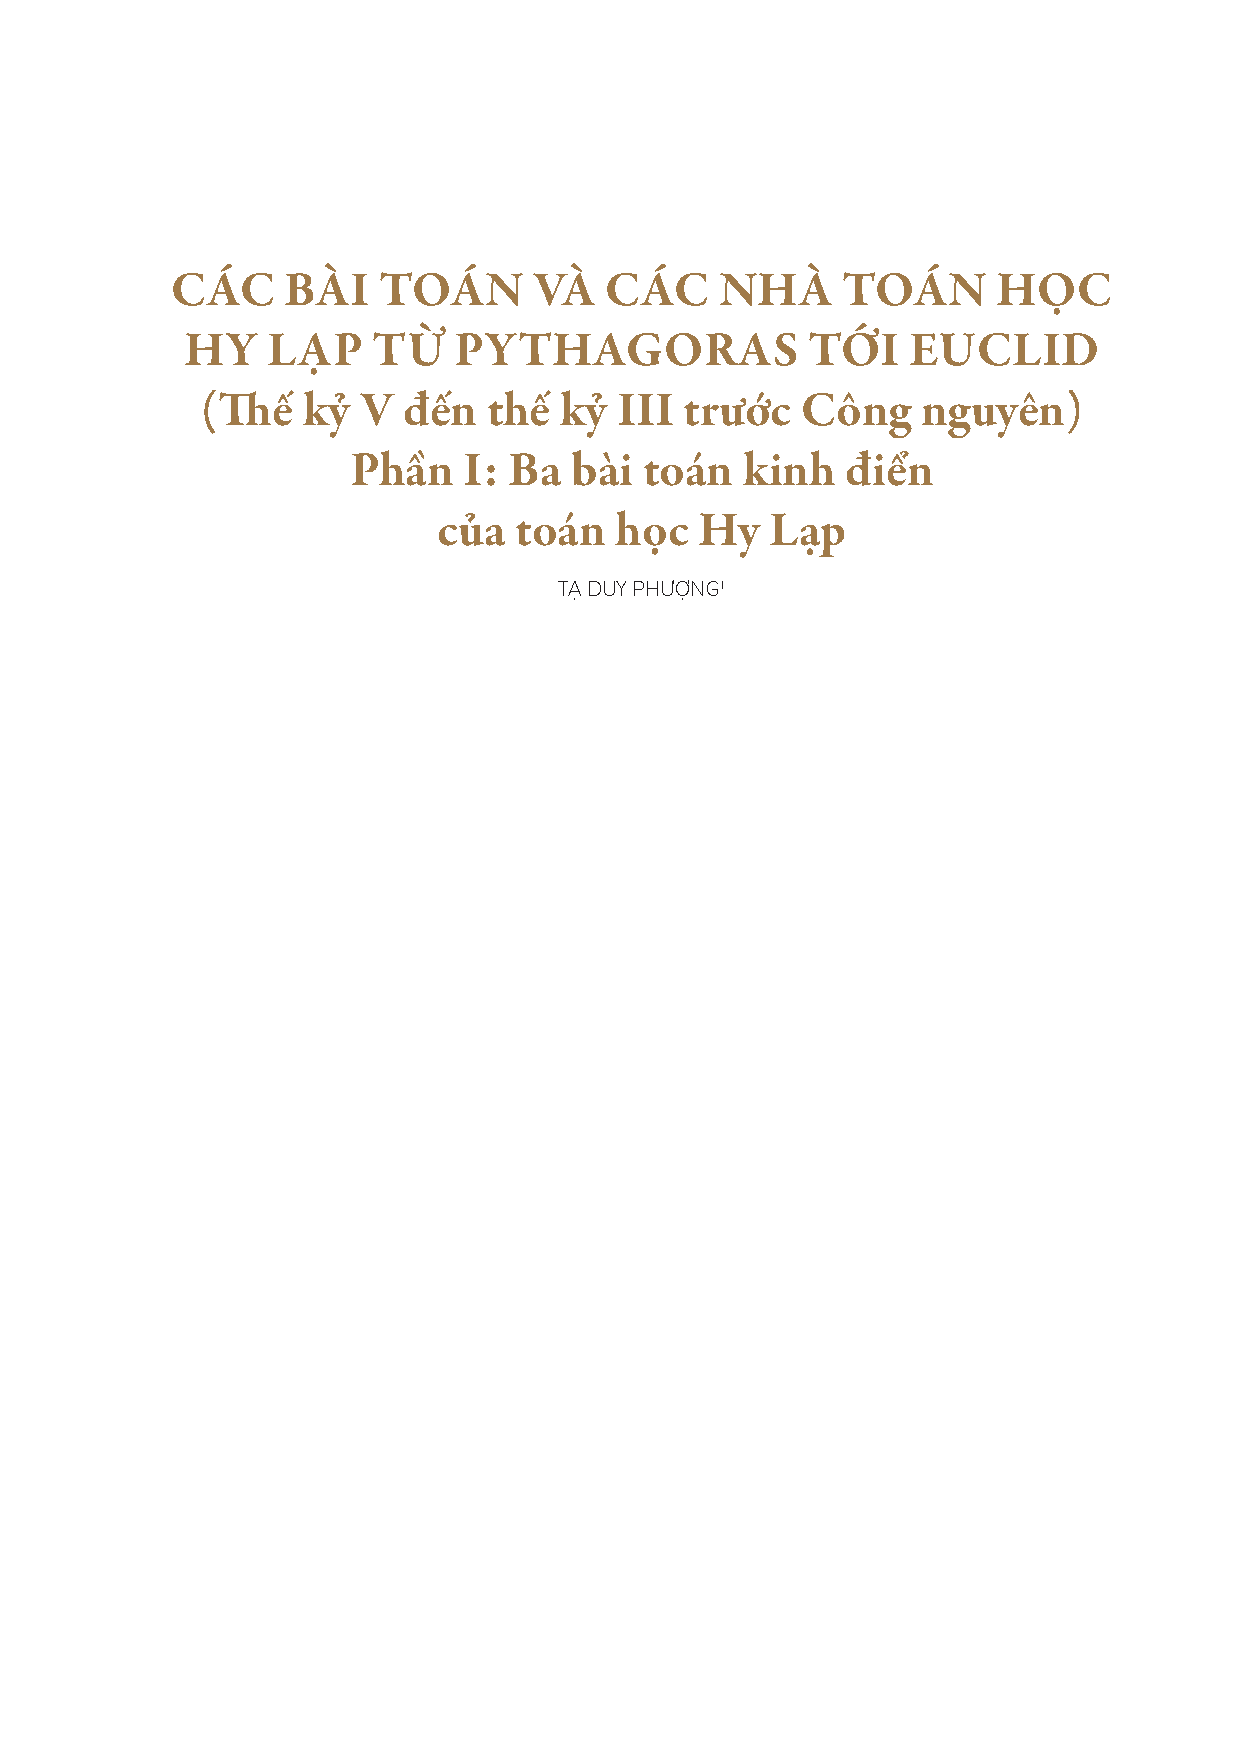
\includegraphics[scale=1]{../tieude.pdf}}}
\centering
\endgroup

\vspace*{235pt}

\begin{multicols}{2}
%	\setlength{\abovedisplayskip}{5pt}
%	\setlength{\belowdisplayskip}{5pt}
	$\pmb{1.}$ \textbf{\color{lichsutoanhoc}Số vô tỷ}
	\vskip 0.05cm
	Hippasus xứ Croton, khoảng $530-450$ trước công nguyên (TCN), ban đầu là người thuộc trường phái Pythagoras, nhưng sau bị khai trừ khỏi trường phái này. Một tài liệu nói những người Pythagoras đã dựng bia mộ ông, như thể ông đã chết; một tài liệu khác nói rằng sự bội đạo của ông đã bị trừng phạt bằng cái chết trên biển trong một tai nạn chìm tàu. Nguyên nhân chính xác có lẽ không bao giờ được biết, do quy tắc bí mật của trường phái Pythagoras, nhưng có ba khả năng đã được nêu ra. 
	\vskip 0.05cm
	Khả năng thứ nhất, Hippasus bị trục xuất vì ông đứng đầu một phong trào dân chủ chống lại những quy định bảo thủ của Pythagoras.
	\vskip 0.05cm
	Khả năng thứ hai quy việc trục xuất ông về lý do ông đã tiết lộ các phát minh của trường phái Pythagoras về ngũ giác đều hoặc khối $12$ mặt đều. 
	\vskip 0.05cm
	Giải thích thứ ba cho rằng ông bị trục xuất vì tiết lộ một khám phá toán học có ý nghĩa tàn khốc đối với học thuyết Pythagoras -- sự tồn tại các số vô tỷ.
	\vskip 0.1cm
	Nguyên lý cơ bản của học thuyết Pythagoras là các thuộc tính của số nguyên hoặc tỷ lệ của chúng (các số hữu tỷ) có thể giải thích bản chất của tất cả mọi thứ, trong hình học cũng như trong thiên văn và xã hội. Tuy nhiên, \textit{Đối thoại} của Plato (khoảng $428-347$ TCN) cho thấy rằng cộng đồng toán học Hy Lạp đã bị choáng váng bởi một tiết lộ hầu như phá hủy toàn bộ niềm tin của người Pythagoras và cộng đồng vào những con số. Đây là khám phá rằng trong bản  thân hình học, các số hữu tỷ không đủ để giải thích các thuộc tính cơ bản. Chẳng hạn, số hữu tỷ không đủ để so sánh tỷ lệ của đường chéo hình vuông, đường chéo hình lập phương hoặc đường chéo ngũ giác đều với cạnh của~nó. 
	\vskip 0.1cm
	Thông thường, người ta cho rằng sự công nhận số vô tỷ liên quan đến ứng dụng của định lý Pythagoras vào tam giác vuông cân. Một chứng minh như vậy rất dễ xây dựng (xem [$10$]). Aristotle ($384-322$ TCN) đã đề cập đến một chứng minh về tính không thông ước$^{\small2}$ của đường chéo của hình vuông với cạnh của nó. Trong chứng minh này, mức độ trừu tượng cao đến mức người ta nghi ngờ nó đã được thực hiện vào thế kỉ V TCN. Tuy nhiên,  khám phá về số vô tỷ có thể đã xảy ra vào thế kỉ V TCN theo những cách khác. 
	\vskip 0.1cm
	\blfootnote{\color{lichsutoanhoc}$^2$Hai đoạn thẳng có độ dài $a$ và $b$ được gọi là thông ước với nhau nếu tồn tại một đoạn thẳng có độ dài $c$ và các số tự nhiên $m$ và $n$ sao cho $a = mc$ và $b = nc$, tức là $\frac{a}{b} = \frac{m}{n}$. Theo ngôn ngữ ngày nay, hai đại lượng là thông ước nếu thương của chúng là một số hữu tỷ.}
	Năm đường chéo của một ngũ giác đều tạo thành một ngũ giác đều nhỏ hơn và các đường chéo của hình ngũ giác thứ hai lần lượt tạo thành hình ngũ giác đều thứ ba ... (Hình $1$).
	\begin{figure}[H]
		\vspace*{-10pt}
		\centering
		\captionsetup{labelformat= empty, justification=centering}
		\begin{tikzpicture}[lichsutoanhoc,scale=0.75]
			\draw  (-1.,1.)-- (2.,1.);
			\draw  (2.,1.)-- (2.9270509831248424,3.85316954888546);
			\draw  (2.9270509831248424,3.85316954888546)-- (0.5,5.616525305762879);
			\draw  (0.5,5.616525305762879)-- (-1.927050983124842,3.853169548885461);
			\draw  (-1.927050983124842,3.853169548885461)-- (-1.,1.);
			\draw  (0.5,5.616525305762879)-- (2.,1.);
			\draw  (0.5,5.616525305762879)-- (-1.,1.);
			\draw  (-1.927050983124842,3.853169548885461)-- (2.9270509831248424,3.85316954888546);
			\draw  (2.9270509831248424,3.85316954888546)-- (-1.,1.);
			\draw  (-1.927050983124842,3.853169548885461)-- (2.,1.);
			\draw  (-0.07294901687515731,3.85316954888546)-- (1.4270509831248426,2.763355756877419);
			\draw  (-0.07294901687515731,3.85316954888546)-- (0.5,2.0898137920080413);
			\draw  (0.5,2.0898137920080413)-- (1.0729490168751583,3.853169548885459);
			\draw  (1.0729490168751583,3.853169548885459)-- (-0.4270509831248419,2.763355756877419);
			\draw  (-0.4270509831248419,2.763355756877419)-- (1.4270509831248426,2.763355756877419);
		\end{tikzpicture}
		\caption{\small\textit{\color{lichsutoanhoc}Hình $1$.}}
		\vspace*{-10pt}
	\end{figure}
	Quá trình này có thể được tiếp tục đến vô hạn, dẫn đến gợi ý: \textit{Tỷ số giữa một đường chéo và một cạnh của một ngũ giác đều không thể là số hữu tỷ.} 
	\vskip 0.1cm
	Xét ngũ giác đều $ABCDE$  với hai đường chéo $AD$  và $BE$  (Hình $2$). Do $\angle ABE = \angle IAE$ và $\angle AEB = \angle IEA$  nên $\Delta ABE \sim \Delta IAE$.  
	\begin{figure}[H]
		\vspace*{-10pt}
		\centering
		\captionsetup{labelformat= empty, justification=centering}
		\begin{tikzpicture}[lichsutoanhoc,scale=0.75]
			\draw  (1.5,4.616525305762879)-- (3.9270509831248424,2.85316954888546);
			\draw  (3.9270509831248424,2.85316954888546)-- (3.,0.);
			\draw  (3.,0.)-- (0.,0.);
			\draw  (0.,0.)-- (-0.9270509831248419,2.853169548885461);
			\draw  (-0.9270509831248419,2.853169548885461)-- (1.5,4.616525305762879);
			\draw  (-0.9270509831248419,2.853169548885461)-- (3.9270509831248424,2.85316954888546);
			\draw  (1.5,4.616525305762879)-- (0.,0.);
	
				\draw [fill=white] (0.,0.) circle (1.5pt);
				\draw (-0.24,-0.23) node {$D$};
				\draw [fill=white] (3.,0.) circle (1.5pt);
				\draw (3.16,-0.23) node {$C$};
				\draw [fill=white] (3.9270509831248424,2.85316954888546) circle (1.5pt);
				\draw (4.06,3.23) node {$B$};
				\draw [fill=white] (1.5,4.616525305762879) circle (1.5pt);
				\draw (1.64,4.99) node {$A$};
				\draw [fill=white] (-0.9270509831248419,2.853169548885461) circle (1.5pt);
				\draw (-1.1,3.29) node {$E$};
				\draw [fill=white] (0.9270509831248427,2.8531695488854605) circle (1.5pt);
				\draw (0.82,3.19) node {$I$};
		\end{tikzpicture}
		\caption{\small\textit{\color{lichsutoanhoc}Hình $2$.}}
		\vspace*{-10pt}
	\end{figure}
	Suy ra $\dfrac{AB}{BE} = \dfrac{IA}{AE}$. Nhưng $AE = AB$  nên 
	\begin{align*}
		&A{B^2} = BE \times IA = BE \times \left( {BE - AB} \right)\\
		\Rightarrow \,& A{B^2} = B{E^2} - BE \times AB.
	\end{align*}
	Chia cả hai vế cho $AB^2$  và đặt $\dfrac{BE}{AB} = x$  ta được $x^2 - x - 1= 0$.  Suy ra $\dfrac{BE}{AB} = x = \dfrac{1 + \sqrt{5}}{2}$. Suy ra $\dfrac{AB}{BE} = \dfrac{1}{x} = \dfrac{\sqrt{5} -1}{2}$. Số $x = \dfrac{1 + \sqrt{5}}{2}$  hoặc $\dfrac{1}{x} = \dfrac{\sqrt{5} - 1}{2}$  được gọi là \textit{tỷ lệ vàng}.
	\vskip 0.1cm
	Có vẻ như, không phải là $\sqrt{2}$  mà là  $\sqrt{5}$ lần đầu tiên tiết lộ sự tồn tại của các số vô tỷ (thông qua các đại lượng không thông ước đến từ ngũ giác đều). Tính chất vô tỷ của tỷ lệ này, trên thực tế, là hệ quả của lập luận được trình bày trên Hình $3$, trong đó tỷ lệ vàng được hiển thị lặp đi lặp lại nhiều lần:
	\begin{align*}
		\frac{{R{P_1}}}{{{P_1}S}} = \frac{{R{P_2}}}{{{P_2}{P_1}}} = \frac{{R{P_3}}}{{{P_3}{P_2}}} = \ldots
	\end{align*}
	\begin{figure}[H]
		\vspace*{-10pt}
		\centering
		\captionsetup{labelformat= empty, justification=centering}
		\begin{tikzpicture}[lichsutoanhoc,scale=0.68]
			\draw  (0.,0.)-- (10.,0.);
				\draw  (0.,0.) -- (0,0.2);
				\draw (0.0,-0.5) node {$R$};
				\draw  (10,0.) -- (10,0.2);
				\draw (10,-0.5) node {$S$};
				\draw  (6.2,0.) -- (6.2,0.2);
				\draw (6.2,-0.5) node {$P_1$};
				\draw  (3.8,0.) -- (3.8,0.2);
				\draw (3.8,-0.5) node {$P_2$};
				\draw  (2.4,0.) -- (2.4,0.2);
				\draw (2.4,-0.5) node {$P_3$};
		\end{tikzpicture}
		\caption{\small\textit{\color{lichsutoanhoc}Hình $3$.}}
		\vspace*{-10pt}
	\end{figure}
	Tính chất này dẫn đến việc tiết lộ, có thể bởi Hippasus, về tính không thông ước giữa đường chéo của ngũ giác đều và cạnh của nó. Không có tài liệu nào khẳng định điều này, nhưng có vẻ như đây là một suy đoán có lý.
	\vskip 0.1cm
	Tỷ lệ giữa đường chéo của hình lập phương với một cạnh bằng $\sqrt{3}$, cũng dẫn tới tính không thông ước của đường chéo và cạnh của hình lập phương, hay tính chất vô tỷ của số $\sqrt{3}$.
	\begin{figure}[H]
		\vspace*{-10pt}
		\centering
		\captionsetup{labelformat= empty, justification=centering}
		\begin{tikzpicture}[lichsutoanhoc,scale=0.8]
			\draw  (0.,0.)-- (4.,0.);
			\draw  (4.,0.)-- (4.,4.);
			\draw  (4.,4.)-- (0.,4.);
			\draw  (0.,4.)-- (0.,0.);
			\draw  (4.,4.)-- (0.,0.);
			\draw  (3.31370849898476,4.)-- (3.3137084989847594,3.3137084989847585);
			\draw  (1.6568542494923808,4.)-- (2.8284271247461903,2.82842712474619);
			
			\draw [fill=white] (0.,0.) circle (1.5pt);
			\draw (-0.2,-0.17) node {$A$};
			\draw [fill=white] (4.,0.) circle (1.5pt);
			\draw (4.22,-0.13) node {$D$};
			\draw [fill=white] (4.,4.) circle (1.5pt);
			\draw (4.16,4.41) node {$C$};
			\draw [fill=white] (0.,4.) circle (1.5pt);
			\draw (-0.16,4.35) node {$B$};
			\draw [fill=white] (1.6568542494923808,4.) circle (1.5pt);
			\draw (1.62,4.41) node {$Q$};
			\draw [fill=white] (3.31370849898476,4.) circle (1.5pt);
			\draw (3.28,4.41) node {$R$};
			\draw [fill=white] (3.31370849898476,4.) circle (1.5pt);
			\draw [fill=white] (3.3137084989847594,3.3137084989847585) circle (1.5pt);
			\draw (3.56,3.05) node {$S$};
			\draw [fill=white] (2.8284271247461903,2.82842712474619) circle (1.5pt);
			\draw (2.86,2.51) node {$P$};
		\end{tikzpicture}
		\caption{\small\textit{\color{lichsutoanhoc}Hình $4$.}}
		\vspace*{-5pt}
	\end{figure}
	Tương tự như ngũ giác đều, nếu trong hình vuông $ABCD$ (Hình $4$) dựng trên đường chéo $AC$ đoạn $AP = AB$  và tại $P$ dựng đoạn thẳng $PQ$  vuông góc với đường chéo thì $\dfrac{CQ}{CP} = \dfrac{AC}{AB}$. Một lần nữa, nếu trên $CQ$  đặt $QR = QP$ và  dựng $RS$  vuông góc với $CR$,  thì  $\dfrac{CS}{CR} = \dfrac{CQ}{CP} = \dfrac{AC}{AB}$. Quá trình này có thể được lặp lại vô hạn. Đây một chứng minh cho thấy không có đơn vị độ dài nào, dù nhỏ, có thể được tìm thấy để đường chéo và cạnh hình vuông là thông ước với nhau.
	\vskip 0.1cm
	\PIbox{\textbf{\color{lichsutoanhoc}Bài tập.} Sử dụng chứng minh $\sqrt{2}$  là số vô tỷ (xem [$10$]), hãy chứng minh $\sqrt{3}$  là số vô tỷ, hay đường chéo của hình lập phương không thông ước với cạnh của nó. Tương tự, chứng minh $\sqrt{5}$ là số vô tỷ.}
	\vskip 0.1cm
	$\pmb{2.}$ \textbf{\color{lichsutoanhoc}Nghịch lý Zeno}
	\vskip 0.1cm
	Học thuyết Pythagoras cho rằng ``Các con số [hữu tỷ] tạo nên toàn bộ thiên đường" thực sự đã phải đối mặt với một vấn đề rất nghiêm trọng khi số vô tỷ được phát hiện, nhưng trường phái Pythagoras còn phải đối mặt với những lập luận do những học giả xứ Elea, một trường phái đối thủ đưa ra. 
	\vskip 0.1cm
	Các nhà triết học Ionia ở Tiểu Á đã tìm cách xác định yếu tố cơ bản của vật chất.
	\vskip 0.1cm
	Thales cho rằng nước là nguồn gốc của vật chất, nhưng những người khác ưu tiên coi không khí hoặc lửa là yếu tố cơ bản. Trường phái Pythagoras đã theo một hướng trừu tượng hơn: cho rằng các con số (hữu tỷ) là cơ bản. Thuyết này, được minh họa một cách tuyệt đẹp trong hình học của các con số tượng hình, đã bị công kích bởi những người theo Parmenides (đầu thế kỉ V TCN) xứ Elea. Nguyên lý cơ bản của trường phái Elea là sự thống nhất và vĩnh viễn, một quan điểm trái ngược với các ý tưởng của Pythagoras về tính đa dạng và thay đổi.  Trong các môn đệ của Parmenides, người được biết đến nhiều nhất là Zeno ở Elea (khoảng $495-430$ TCN), người đã đưa ra các lý lẽ để chứng minh sự mâu thuẫn trong các khái niệm của Pythagoras.
	\vskip 0.1cm
	Những người Pythagoras cho rằng không gian và thời gian có thể được coi là bao gồm các điểm và cá thể, nhưng không gian và thời gian cũng có thuộc tính, được gọi là ``tính liên tục". 
	Một mặt, tính liên tục có các đặc điểm của đơn vị hình học -- điểm -- và mặt khác, có các đặc điểm của các đơn vị số hoặc các số.
	Aristotle ($384-322$ TCN) đã mô tả quan điểm của Pythagoras là ``sự thống nhất có vị trí" hoặc ``sự thống nhất được xem xét trong không gian". 
	Để chống lại quan điểm này, Zeno đưa ra những nghịch lý, trong đó các nghịch lý về chuyển động dường như đã gây ra nhiều rắc rối nhất:
	\vskip 0.1cm
	$(1)$ Sự phân đôi (the Dichotomy), 
	\vskip 0.1cm
	$(2)$ Achilles và con rùa, 
	\vskip 0.1cm
	$(3)$ Mũi tên (the Arrow), và 
	\vskip 0.1cm
	$(4)$ Sân vận động (the Stade, hay Stadium).
	\vskip 0.1cm
	\textbf{\color{lichsutoanhoc}Sự phân đôi}
	\vskip 0.1cm
	Một người chạy được một quãng đường nhất định, trước tiên anh ta phải đi một nửa quãng đường này, nhưng trước khi anh ta có thể làm được điều này, anh ta phải đi một phần tư quãng đường đầu tiên, và trước đó, một phần tám quãng đường đầu tiên, và cứ như vậy, thông qua vô số đoạn.  Anh ta phải tạo vô số đoạn trong một thời gian hữu hạn, nhưng điều này là không thể. Do đó sự khởi động của chuyển động là không thể.
	\vskip 0.1cm
	\textbf{\color{lichsutoanhoc}Achilles và con rùa}
	\vskip 0.1cm
	Nghịch lý thứ hai tương tự như nghịch lý thứ nhất, ngoại trừ việc chia nhỏ vô hạn không gian là lũy tiến, chứ không phải là thoái lui. Giả sử Achilles chạy đua với một con rùa đã xuất phát từ trước. Khi Achilles đạt đến vị trí ban đầu của con rùa, thì con rùa đã đi được một đoạn ngắn và vào thời điểm Achilles vượt qua đoạn này, con rùa sẽ tiến lên hơi xa hơn, và quá trình này tiếp tục vô hạn, với kết quả là Achilles nhanh nhẹn không bao giờ có thể vượt qua con rùa chậm chạp.
	\vskip 0.1cm
	\textbf{\color{lichsutoanhoc}Mũi tên}
	\vskip 0.05cm
	Các nghịch lý \textit{Phân đôi} và \textit{Achilles} lập luận rằng chuyển động là không thể dưới giả thiết về sự chia nhỏ vô hạn không gian và thời gian. Mặt khác, \textit{Mũi tên} và \textit{Sân vận động} lập luận rằng chuyển động không thể xảy ra nếu giả định ngược lại rằng có một đại lượng nhỏ nhất của không gian và thời gian. Trong \textit{Mũi tên}, Zeno lập luận rằng một vật thể đang bay luôn chiếm một khoảng không gian bằng chính nó, nhưng chiếm một khoảng không gian bằng chính nó thì nó không chuyển động. Vì thế mũi tên đang bay luôn dừng lại, do đó chuyển động của nó chỉ là một ảo giác.
	\vskip 0.05cm
	\textbf{\color{lichsutoanhoc}Sân vận động}
	\vskip 0.05cm
	Gây tranh cãi nhiều nhất và khó xử nhất về những nghịch lý trong chuyển động là \textit{Sân vận động}, nó có thể được diễn giải như sau. 
	\vskip 0.1cm
	Giả sử rằng tại một thời điểm nhất định, các vật ${A_1}$, ${A_2}$, ${A_3}$, ${A_4}$, ${A_5}$, ${A_6}$, $A_7$, $A_8$; $B_1$, $B_2$, $B_3$, $B_4$, $B_5$, $B_6$, $B_7$, $B_8$  và $C_1$, $C_3$, $C_3,$ $C_4$, $C_5$, $C_6$, $C_7$, $C_8$ chiếm các vị trí tương đối sau \linebreak(Hình $5a$):
	\begin{figure}[H]
		\vspace*{-10pt}
		\centering
		\captionsetup{labelformat= empty, justification=centering}
		\begin{tikzpicture}[scale=0.44,lichsutoanhoc,node font=\scriptsize]
			\draw (0,0) grid (8,1);
			\draw (0,2) grid (-8,3);
			\draw (-4,4) grid (4,5);
			\draw[-stealth] (-1,0.5) -- (-3, 0.5);
			\draw[-stealth] (1,2.5) -- (3, 2.5);

			\foreach \x in {1,2,...,8}{
				\node at (\x-0.5, 0.5) {$C_\x$};
				\node at (\x - 4.5, 4.5) {$A_\x$};
				\node at (-\x + 0.5, 2.5) {$B_\x$};}
		\end{tikzpicture}
		\caption{\small\textit{\color{lichsutoanhoc}Hình $5a$: Sân vận động.}}
		\vspace*{-10pt}
	\end{figure}
	Các vật $B$ chuyển động sang phải và các vật $C$ chuyển động sang trái với cùng vận tốc để được Hình $5b$:
	\begin{figure}[H]
	\vspace*{-10pt}
	\centering
	\captionsetup{labelformat= empty, justification=centering}
	\begin{tikzpicture}[scale=0.45,lichsutoanhoc,node font=\scriptsize]
		\draw (0,0) grid (8,1);
		\draw (0,2) grid (8,3);
		\draw (0,4) grid (8,5);
		
		\foreach \x in {1,2,...,8}{
			\node at (\x-0.5, 0.5) {$C_\x$};
			\node at (\x-0.5, 4.5) {$A_\x$};
			\node at (8.5-\x, 2.5) {$B_\x$};}
	\end{tikzpicture}
	\caption{\small\textit{\color{lichsutoanhoc}Hình $5b$: Sân vận động.}}
	\vspace*{-5pt}
	\end{figure}
	Khi $C_1$  đi qua $8$ vật $B$  (và $B_1$ đi qua 8 vật  $C$) thì $B_1$  chỉ đi qua $4$ vật $A_5, A_6, A_7, A_8$  (tương tự,  $C_1$  đi qua $4$ vật  $A_1, A_2, A_3, A_4$). Nhưng $C_1$  mất cùng một thời gian khi đi qua $8$ vật  $B$ như là đi qua $4$ vật $A$.  Suy ra thời gian để  $C_1$  đi qua $8$ vật $A$  cũng bằng thời gian đi qua một nửa $A$,  hay thời gian đã cho bằng một nửa của nó. Mâu thuẫn.     
	\vskip 0.1cm
	Aristotle cho rằng Zeno đã không hiểu sự khác nhau giữa chuyển động tương đối với chuyển động tuyệt đối và tin rằng ông đã bác bỏ nghịch lý của Zeno vì ông đã phủ nhận giả định ban đầu: thời gian bao gồm các đơn vị không thể phân chia. Tuy nhiên, giải thích thấu đáo nghịch lý Zeno về sân vận động chỉ được đưa ra bởi Brochard, Noël và Russell vào thế kỉ XIX--XX.
	\vskip 0.1cm 
	Các lập luận của Zeno dường như đã có ảnh hưởng sâu sắc đến sự phát triển của toán học Hy Lạp, có thể so sánh với sự phát hiện ra số vô tỉ, mà chúng có thể có liên quan với nhau. Ban đầu, trong lý thuyết của Pythagoras, độ lớn được biểu thị bằng hạt hoặc đá cuội, nhưng đến thời Euclid thì có một sự thay đổi hoàn toàn về quan điểm.  Độ lớn nói chung không phải được liên kết với các con số hoặc viên sỏi, mà với các đoạn thẳng. Trong \textit{Cơ sở}, thậm chí các số nguyên cũng được biểu diễn bằng các đoạn. Vương quốc của con số có đặc tính rời rạc, nhưng thế giới của các đại lượng liên tục là một thứ ngoài số và phải được xử lý bằng phương pháp hình học (và điều này bao gồm hầu hết toán học thời kỳ tiền cổ đại và Pythagoras).  Dường như là hình học, hơn là con số, thống trị thế giới.
%	\vskip 0.1cm
%	$\pmb{3.}$ \textbf{\color{lichsutoanhoc}Học viện Plato}
%	\vskip 0.1cm
%	Thế kỷ thứ tư TCN đã mở đầu bằng cái chết của Socrates (khoảng $470-399$ TCN), một học giả đã áp dụng phương pháp biện chứng của Zeno và bác bỏ thuyết Pythagoras của Archytas (khoảng $420-347$ TCN). Socrates thừa nhận rằng khi còn trẻ, ông đã bị thu hút bởi những câu hỏi như tại sao tổng $2 + 2$ lại bằng tích $2 \times 2$  nhưng khi nhận ra rằng cả toán học và khoa học đều không thể thỏa mãn mong muốn của ông để  hiểu bản chất của sự vật, ông đã tự nghiên cứu để hiểu những điều bản chất.
%	\end{multicols}
%	\begin{figure}[H]
%		\vspace*{5pt}
%		\centering
%		\captionsetup{labelformat= empty, justification=centering}
%		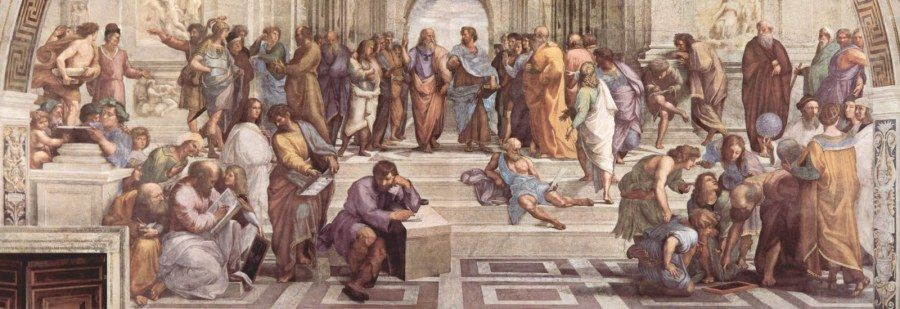
\includegraphics[width= 1\linewidth]{H7}
%		\caption{\small\textit{\color{lichsutoanhoc}Hình $6$: The School of Athens của Rafael tại Vaticant.}}
%		\vspace*{-10pt}
%	\end{figure}
%	\begin{multicols}{2}
%	Trong \textit{Phaedo} của Plato, cuộc đối thoại trong đó những giờ cuối cùng của Socrates được mô tả rất đẹp, chúng ta thấy những nghi ngờ siêu hình sâu sắc như thế nào loại trừ mối quan tâm của Socrate về toán học hoặc khoa học tự nhiên:
%	\vskip 0.1cm
%	\textit{Tôi không thể tự thỏa mãn bản thân rằng, khi một cái được thêm vào một cái, mà phép cộng được thực hiện trở thành hai. 
%	\vskip 0.1cm
%	Tôi không thể hiểu làm thế nào khi tách khỏi nhau, mỗi trong số chúng là một chứ không phải hai, và bây giờ, khi chúng được kết hợp lại với nhau, chỉ là sự đặt cạnh nhau, là nguyên nhân khiến chúng trở thành hai.}
%	\vskip 0.1cm
%	Do đó, ảnh hưởng của Socrates trong sự phát triển của toán học là không đáng kể, nếu không nói là tiêu cực. Điều đáng ngạc nhiên là chính học trò và người ngưỡng mộ ông là Plato đã trở thành cảm hứng toán học của thế kỷ thứ tư TCN. 
%	\vskip 0.1cm
%	Mặc dù bản thân Plato không có đóng góp kết quả toán học nổi bật cụ thể nào, nhưng ông đã là trung tâm của hoạt động toán học thời gian đó, hướng dẫn và truyền cảm hứng cho sự phát triển của toán học. Tại cửa trường học của ông, Học viện (The Academy) ở Athens, được khắc khẩu hiệu ``Ai không biết hình học không vào đây".
%	\vskip 0.1cm
%	\PIbox{ΑΓΕΩΜΕΤΡΗΤΟΣ ΜΗΔΕΙΣ ΕΙΣΙΤΩ.}
%	\vskip 0.1cm
%	Sự nhiệt tình của Plato đối với toán học khiến ông được biết đến không phải với tư cách là một nhà toán học, mà là ``người tạo ra các nhà toán học".
%	\vskip 0.1cm
%	Sáu nhà toán học (ngoài Plato và Aristotle) sống giữa năm mất của Socrates ($399$ TCN) và năm mất của Aristotle ($322$ TCN) -- gồm Theodorus xứ Cyrene (thế kỉ V TCN), Theaetetus (khoảng $414-369$ TCN), Eudoxus xứ Cnidus (khoảng $410-347$ TCN), hai anh em Menaechmus ($380-320$ TCN) và Dinostratus ($390-320$  TCN), và Autolycus xứ Pitane ($360-320$ TCN) -- là những nhà toán học đã có liên kết ít nhiều chặt chẽ với Học viện Plato.
%	\vskip 0.1cm
%	Rõ ràng là việc Plato rất coi trọng toán học không đến từ Socrates. Trên thực tế, các bài giảng trong thời kỳ đầu và tác phẩm Đối thoại (Dialogues) của Plato hiếm khi đề cập đến toán học. Archytas, một người bạn của Plato, là người đã khiến Plato quan tâm đến toán học, khi Ông đến thăm bạn ở Sicily vào năm $388$ TCN. Có lẽ chính khi đó, Plato mới biết đến năm hình đa diện đều, được liên kết với bốn nguyên tố (nước, lửa, không khí và đất) của Empedocles ($490-430$ TCN) trong một sơ đồ vũ trụ đã mê hoặc các nhà nghiên cứu trong nhiều thế kỉ (Hình $7$). 
%	\vskip 0.1cm
%	Có thể, sự coi trọng của Pythagoras đối với khối $12$ mặt đều đã khiến Plato xem xét nó, khối đa diện đều thứ năm và cuối cùng, như một biểu tượng của vũ trụ. 
%	Plato đặt ý tưởng của ông về đa diện đều thành một cuộc đối thoại có tiêu đề \textit{Timaeus}, được đặt tên cho một người đóng vai trò là người đối thoại chính thuộc trường phái Pythagoras. Không biết Timaeus xứ Locri có thực sự tồn tại không, hay Plato đã phát minh ra Timaeus như một nhân vật để thể hiện quan điểm của Pythagoras, khi ấy vẫn còn mạnh mẽ ở khu vực mà ngày nay là nước Ý. 
%	\begin{figure}[H]
%		\vspace*{-5pt}
%		\centering
%		\captionsetup{labelformat= empty, justification=centering}
%		\begin{tikzpicture}[scale=0.8, lichsutoanhoc, node font=\small]
%			\draw  (0.,0.)-- (3.,3.);
%			\draw  (3.,3.)-- (0.,6.);
%			\draw  (0.,6.)-- (-3.,3.);
%			\draw  (-3.,3.)-- (0.,0.);
%			\draw [dashed] (0.,0.)-- (0.,6.);
%			\draw [dashed] (-3.,3.)-- (3.,3.);
%			\draw[color=black] (1.9,1.45) node {\color{lichsutoanhoc}Ẩm};
%			\draw[color=black] (1.8,4.91) node {\color{lichsutoanhoc}Nóng};
%			\draw[color=black] (-1.75,4.91) node {\color{lichsutoanhoc}Khô};
%			\draw[color=black] (-1.95,1.33) node {\color{lichsutoanhoc}Lạnh};
%			\draw(0,6) node[above] {Lửa -- Tứ diện đều};
%			\draw(0,0) node[below] {Nước -- Khối $20$ mặt đều};
%			\draw(3.4,3) node[rotate=-90] {Đất -- Lập phương};
%			\draw(-3.2,3) node[rotate=90] {Không Khí -- Bát diện đều};
%		\end{tikzpicture}
%		\caption{\small\textit{\color{lichsutoanhoc}Hình $7$: Sơ đồ vũ trụ ứng với khối đa diện.}}
%		\vspace*{-10pt}
%	\end{figure}
%	Các khối đa diện đều thường được gọi là ``vật thể vũ trụ" hoặc ``khối đa diện Plato" bởi vì cách mà Plato trong \textit{Timaeus} đã áp dụng chúng vào giải thích các hiện tượng khoa học.
%	\vskip 0.1cm
%	Mặc dù đối thoại này, có lẽ được viết khi Plato đã gần bảy mươi tuổi, cung cấp bằng chứng xác thực sớm nhất cho sự liên kết của bốn nguyên tố với khối đa diện đều, phần lớn sự tưởng tượng này có thể là do trường phái Pythagoras.
%	\vskip 0.1cm
%	Proclus (khoảng $410-485$) quy việc xây dựng hình học vũ trụ cho Pythagoras, nhưng có thể bạn của Plato là Theaetetus (khoảng $414-369$ TCN) đã viết về liên kết giữa vũ trụ và khối đa diện đều. 
%	\vskip 0.1cm
%	Quyển XIII của \textit{Cơ sở} của Euclid nói rằng chỉ có ba trong số năm khối đa diện là do Pythagoras, và nhờ Theaetetus mà khối bát diện và hai mươi mặt đều đã được biết đến.
%	\vskip 0.1cm
%	Có vẻ như Theaetetus đã thực hiện một trong những nghiên cứu quy mô nhất về năm khối đa diện, và định lý nói rằng có và chỉ có năm khối đa diện đều là thuộc về Theaetetus. Có lẽ ông cũng là tác giả của các tính toán về tỷ lệ các cạnh của khối đa diện đều và bán kính mặt cầu ngoại tiếp. 
%	\vskip 0.1cm
%	Theaetetus là một thanh niên Athens chết vì bệnh kiết lỵ kết hợp với vết thương trong trận chiến, và cuộc đối thoại của Plato mang tên ông là một sự tưởng nhớ của Plato đối với người bạn của mình.
%	\vskip 0.1cm
%	Trong cuộc đối thoại, có bối cảnh trước đó khoảng ba mươi năm, Theaetetus thảo luận với Socrates và Theodorus về bản chất của các đại lượng vô ước với nhau (hay các đại lượng không thông ước với nhau). Người ta đã giả định rằng cuộc thảo luận này phần nào có dạng mà chúng ta tìm thấy trong phần mở đầu của Quyển X của \textit{Cơ sở}.
%	\vskip 0.1cm
%	Ở đây, sự phân biệt không chỉ được thực hiện giữa các đại lượng thông ước và vô ước, mà còn giữa các đại lượng khi độ dài là vô ước với nhau, nhưng có diện tích thông ước với nhau. Như $\sqrt{3}$  và $\sqrt{5}$  không thông ước về độ dài, nhưng thông ước về diện tích, vì các hình vuông của chúng có tỷ lệ là $3/5$.
%	\vskip 0.1cm
%	Mặt khác, các đại lượng  $\sqrt{1 + \sqrt{3}}$  và $\sqrt{1 + \sqrt{5}}$ là không thông ước cả về độ dài và diện tích.
%	\vskip 0.1cm
%	Cuộc đối thoại mà Plato sáng tác để tưởng nhớ người bạn Theaeteus của mình chứa thông tin về một nhà toán học khác, Theodorus xứ Cyrene, thầy của Plato và Theaetetus, người mà Plato ngưỡng mộ và là người đã đóng góp vào sự phát triển của lý thuyết về các đại lượng vô ước. 
%	\vskip 0.1cm
%	Không biết bằng cách nào mà Theodorus đã làm điều này và tại sao ông lại dừng lại ở $\sqrt{17}$ 
%	\vskip 0.1cm
%	Theodorus là người đầu tiên chứng minh tính vô tỷ của căn bậc hai của các số nguyên không chính phương từ $3$ đến $17$.	 
%	\vskip 0.1cm
%	Chứng minh, trong mọi trường hợp, được đưa ra bởi Aristotle khi ông xây dựng trục xoắn ốc dọc theo đoạn $\sqrt{2}$. Các tác phẩm lịch sử cổ đại chỉ ra rằng Theodorus đã khám phá ra điều này và sau này nó được đưa vào \textit{Cơ sở}, nhưng các tác phẩm của Theodorus đã bị mất. 
%	\begin{figure}[H]
%		\vspace*{-5pt}
%		\centering
%		\captionsetup{labelformat= empty, justification=centering}
%		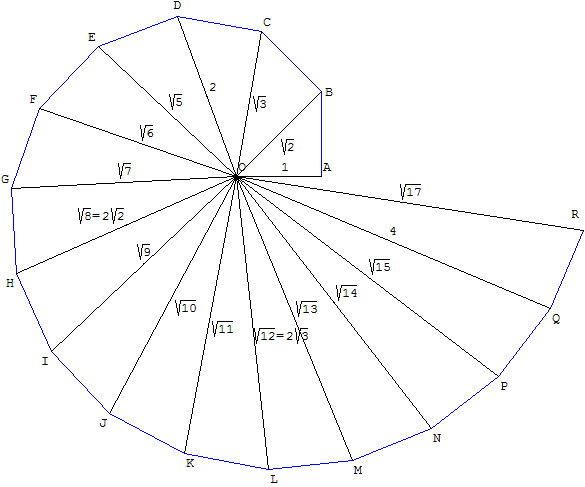
\includegraphics[width= 0.85\linewidth]{H8}
%		\caption{\small\textit{\color{lichsutoanhoc}Hình $8$: Xoắn ốc Theodorus.}}
%		\vspace*{-10pt}
%	\end{figure}
%	Plato có vai trò quan trọng trong lịch sử toán học phần lớn vì ông là người truyền cảm hứng và là người sáng lập Học viện đào tạo ra nhiều nhà toán học, cũng như do sự nhạy bén của ông về sự phân biệt ở Hy Lạp cổ đại giữa số học (theo nghĩa của lý thuyết về các con số) và kỹ thuật tính toán. 
%	\vskip 0.1cm
%	Plato cho rằng toán học là cần thiết cho doanh nhân và quân sự, ``phải học nghệ thuật của những con số, nếu không anh ta sẽ không biết cách dàn quân".
%	\vskip 0.1cm
%	Mặt khác, nhà triết học phải là một nhà số học ``bởi vì anh ta phải nhảy ra khỏi biển của những thay đổi và nắm giữ bản thể đích thực." Hơn nữa, Plato nói trong tác phẩm \textit{Cộng hòa (The Republic)}: ``Số học có tác dụng rất lớn và nâng cao, buộc tâm trí nghĩ về số trừu tượng."
%	\vskip 0.1cm 
%	Trong số học, Plato đã nhìn thấy một hố ngăn cách lý thuyết và các khía cạnh tính toán, cũng như trong hình học, ông cũng tán thành toán học thuần túy chống lại quan điểm duy vật.  
%	\vskip 0.1cm
%	Bất kỳ một trong số vô số đường kính của đường tròn là trục đối xứng của hình. Bất cứ điểm nào trên một đường thẳng kéo dài vô hạn có thể được coi là tâm của đối xứng, giống như bất kỳ đường thẳng nào vuông góc với đường thẳng đã cho là trục đối xứng của đường thẳng đã cho. Triết học Plato, với sự áp dụng các ý tưởng của nó, tự nhiên sẽ tìm thấy vai trò của đường thẳng và đường tròn giữa các hình hình học. Tương tự, Plato tôn vinh tam giác.
%	\vskip 0.1cm 
%	Sự liên kết của bốn khối đa diện đầu tiên với bốn yếu tố phổ quát truyền thống của vũ trụ đã cung cấp cho Plato trong \textit{Timaeus}  một lý thuyết thống nhất tuyệt đẹp về vật chất, theo đó mọi thứ đều được xây dựng bằng các tam giác vuông lý tưởng. Toàn bộ sinh lý học, cũng như khoa học về chất trơ, dựa trên các hình tam giác.
%	\vskip 0.1cm
%	Pythagoras nổi tiếng là người đã thiết lập toán học như một chủ đề tự do, nhưng Plato đã có ảnh hưởng trong việc làm cho toán học trở thành một phần thiết yếu của chương trình đào tạo.
%	\vskip 0.1cm
%	Có lẽ bị ảnh hưởng bởi Archytas, Plato đã thêm vào các chủ đề ban đầu trong bộ bốn (quadrivium: Số học, Hình học, Âm nhạc, Thiên văn) một môn học mới: Hình học không gian, vì ông tin rằng hình học không gian đã không được nhấn mạnh đầy đủ. Plato cũng thảo luận về nền tảng của toán học, làm rõ một số định nghĩa và xây dựng lại các giả thiết. Ông nhấn mạnh rằng lý luận được sử dụng trong hình học không đề cập đến những con số hữu hình mô tả chúng, mà là những ý tưởng tuyệt đối mà chúng đại diện. 
%	\vskip 0.1cm
%	Những người theo thuyết Pythagoras đã định nghĩa điểm là ``sự thống nhất có vị trí," nhưng Plato lại nghĩ về nó như là sự khởi đầu của một đường thẳng.
%	\vskip 0.1cm 
%	Định nghĩa của một đường là ``chiều dài không có chiều rộng" dường như bắt nguồn từ trường phái Plato.
%	\vskip 0.1cm
%	Trong số học, Plato không chỉ nhấn mạnh sự phân biệt giữa số lẻ và số chẵn, mà còn là các loại ``chẵn nhân chẵn", ``chẵn nhân lẻ" và ``lẻ nhân lẻ". Mặc dù ta biết rằng Plato đã thêm vào các tiên đề của toán học, chúng ta không có một cơ sở nào để khẳng định điều này.
%	\vskip 0.1cm
%	Rất ít đóng góp toán học cụ thể được quy cho Plato. Một công thức cho bộ ba Pythagoras -- ${(2n)^2} + {({n^2} - 1)^2} = {({n^2} + 1)^2}$, trong đó  $n$ là số tự nhiên bất kỳ -- mang tên Plato, nhưng đây chỉ là một phiên bản sửa đổi của kết quả được người Babylon và người Pythagoras đã biết. 
%	\vskip 0.1cm
%	Có lẽ thực sự có ý nghĩa quan trọng hơn cả trong những thứ được gán cho Plato là cái gọi là phương pháp phân tích (analytic method).
%	\vskip 0.1cm
%	Trong chứng minh toán học, ta bắt đầu với những gì đã cho, và từ các tiên đề và các định đề. Tiến hành từng bước một, sau đó đến khẳng định cần được chứng minh.
%	\vskip 0.1cm
%	Plato dường như đã chỉ ra rằng  về mặt sư phạm, khi không tìm được một chuỗi lý luận hiển nhiên từ giả thiết đến kết luận, thường là thuận tiện hơn nếu ta bắt đầu bằng mệnh đề cần được chứng minh và từ đó suy ra một kết luận được biết là đúng. Nếu, sau đó, có thể đảo ngược các bước trong chuỗi lý luận này, kết quả sẽ là mệnh đề đã được chứng minh.
%	\vskip 0.1cm
%	Plato không hẳn là người đầu tiên nêu lên quan điểm phân tích.  Nhưng những gì Plato có thể đã làm là chính thức hóa quá trình này, hoặc có thể ông đã đặt tên cho nó.
%	\vskip 0.1cm
%	Vai trò của Plato trong lịch sử toán học vẫn còn bị tranh cãi gay gắt. Một số người coi ông là một nhà tư tưởng đặc biệt sâu sắc và nhạy bén. Những người khác hình dung ông như một người đã thu hút các nhà toán học theo con đường lí luận trừu tượng, đi xa những vấn đề thực tiễn. 
%	\vskip 0.1cm
%	Trong mọi trường hợp, ít ai có thể phủ nhận rằng Plato đã có tác động to lớn đối với sự phát triển của toán học. Học viện Plato ở Athens trở thành trung tâm toán học của thế giới, và từ ngôi trường này, xuất hiện các giáo viên và nghiên cứu viên hàng đầu đến vào giữa thế kỷ thứ tư TCN. Trong số này, nổi tiếng nhất là Eudoxus xứ Cnidus (khoảng $408-335$ TCN),  một học trò của Plato và người đã trở thành nhà toán học và nhà thiên văn học nổi tiếng nhất trong thời đại của mình.
%	\vskip 0.1cm
%	\textbf{\color{lichsutoanhoc}Tài liệu chính dùng để soạn}
%	\vskip 0.1cm
%	[$1$] David M. Burton, \textit{The History of Mathematics, An Introduction}, Seventh Edition, McGraw--Hill, $2011$. Chapter $3$: The Beginnings of Greek Mathematics, pp. $116-139$.
%	\vskip 0.1cm
%	[$2$] Euclid’s \textit{Elements of Geometry}, edited and provided with a modern English translation by Richard Fitzpatrick, Independently published, $2008$, $544$ p.
%	\vskip 0.1cm
%	[$3$] David Fowler, \textit{The Mathematics of Plato’s Academy}, Second Edition, Clarendon Press, Oxford, $1999$, $441$ p.
%	\vskip 0.1cm   
%	[$4$] Thomas Heath, \textit{A History of Greek Mathematics}, Oxford at the Clarendon Press, $1921$, Volume $1$: From Thales to Euclid, pp. $170-315$.
%	\vskip 0.1cm   
%	[$5$] Victor J. Katz, \textit{A History of Mathematics, An Introduction}, Third Edition, Addison--Wesley, $2009$. Chapter $2$: \textit{The Beginnings of Mathematics in Greek}, pp. $40-49$.
%	\vskip 0.1cm
%	[$6$] Uta C. Merzbach and Carl B. Boyer, \textit{A
%	History of Mathematics}, Third Edition, John Wiley \& Sons, $2011$, pp. $65-80$.
%	\vskip 0.1cm
%	[$7$] George Johston Allman, \textit{Greek Geometry, From Thales to Euclid}, Dublin Universty Press, $1885$, $432$ p.
%	\vskip 0.1cm  
%	[$8$] R. Lloyd, \textit{Early Greek Science: Thales to Aristotle}, $1970$, Chatto \& Windus, London, $156$ p.
%	\vskip 0.1cm 
%	[$9$] Arpad Szabo, \textit{The beginnings of Greek Mathematics}, Springer, $1978$, $363$ p.
	\vskip 0.1cm
	\textbf{\color{lichsutoanhoc}Tài liệu trích dẫn}
	\vskip 0.1cm
	[$10$] Tạ Duy Phượng, \textit{Pythagoras và trường phái toán học Pythagoras}, Tạp chí Pi, Tập $6$ ($2022$), số $5$, trang $45-53$.
\end{multicols}